\documentclass[a4paper,11pt]{article}
\usepackage[utf8]{inputenc}
\usepackage[czech]{babel}
\usepackage{times}

\usepackage{array}
\usepackage{multirow}
\usepackage[paper=portrait,pagesize]{typearea}
\usepackage[czech,ruled,linesnumbered,noline,longend]{algorithm2e}
\usepackage{geometry}
    \geometry{
    a4paper,
    total={17cm,24cm},
    left=2cm,
    top=3cm,
    }
\usepackage{picture}
\usepackage{graphics}
\usepackage{pdflscape}

\begin{document}
\begin{titlepage}

\begin{center}
    \Huge
        \textsc{Vysoké učení technické v Brně}\\
    \huge
        \textsc {Fakulta informačních technologií} 
        \vspace{\stretch{0.382}}

    \LARGE
        Typografie a publikování -- 2. projekt \\
    \Huge
        Tabulky a obrázky \\
        \vspace{\stretch{0.618}}
\end{center}

{\LARGE 4.4.2021 \hfill
Tomáš Juhász (xjuhas04)}
\end{titlepage}

\section{Úvodní strana}
    Název práce umístěte do zlatého řezu a nezapomeňte uvést dnešní datum a vaše jméno příjmení.
\section{Tabulky}
    Pro sázení tabulek můžeme použít bud’ prostředí \texttt{tabbing} nebo prostředí \texttt{tabular}.
    \subsection{Prostředí tabbing}
        Při použití \texttt{tabbing} vypadá tabulka následovně:
        \begin{tabbing}
                Vodní melouny\quad \=\textbf{Cena} \quad \= \textbf{Množství}  \quad  \kill
                \textbf{Ovoce}    \> \textbf{Cena}    \> \textbf{Množství}  \\
                Jablka            \> 25,90            \> 3 kg     \\
                Hrušky            \> 27,40            \> 2,5 kg   \\
                Vodní melouny     \> 35,-             \> 1 kus    \\
        \end{tabbing}
        Toto prostředí se dá také použít pro sázení algoritmů, ovšem vhodnější je použít prostředí \texttt{algorithm} nebo \texttt{algorithm2e} (viz sekce \ref{algorithm_sec})
    \subsection{Prostředí tabular}
        Další možností, jak vytvořit tabulku, je použít prostředí \texttt{tabular}. Tabulky pak budou vypadat takto\footnote{Kdyby byl problem s \texttt{cline}, zkuste se podívat  třeba sem: http://www.abclinuxu.cz/tex/poradna/show/325037}:
\begin{table}[h] 
\centering 
\catcode`\-=12

\begin{tabular}{|c|c|c|}
\hline 
 & \multicolumn{2}{c |}{\bfseries{Cena}} \\\cline {2-3}
 \bfseries{Měna} & \bfseries{nákup} & \bfseries{prodej}  \\ 
    \hline 
\multirow{3}{*}{}
     EUR  &  25,227 & 26,943  \\
     GBP  &  29,368 & 31,492  \\
     USD  &  21,260 & 22,661   \\
  \hline 
    \end{tabular}
    \caption{\label{tab:tab1}Tabulka kurzů k dnešnímu dni}
    \label{currency}

\end{table}

\begin{table}[h] 
\centering 
\catcode`\-=12

\begin{tabular}{|>{\bfseries}c|c|}
    \hline
        $A$ & $\neg A$\\
    \hline
         P & N\\
         O & X\\
         X & X\\
         N & P\\
    \hline
\end{tabular}
\begin{tabular}{|c|c|c|c|c|c|}
\hline 
    \multicolumn{2}{|c|}{\multirow{2}{*}{$A \land B$}}&\multicolumn{4}{|c|}{$B$}\\\cline{3-6}
    \multicolumn{2}{|c|}{} & \textbf{P} & \textbf{O} & \textbf{X} & \textbf{N} \\ 
\hline 
\multirow{4}{*}{$A$}
    & \textbf{P}  &  P & O & X & N  \\\cline{2-6} 
    & \textbf{O}  &  O & O & N & N  \\\cline{2-6}
    & \textbf{X}  &  X & N & X & N  \\\cline{2-6}
    & \textbf{N}  &  N & N & N & N  \\\cline{2-6}
  \hline 
\end{tabular}
\begin{tabular}{|c|c|c|c|c|c|}
\hline 
    \multicolumn{2}{|c|}{\multirow{2}{*}{$A \lor B$}}&\multicolumn{4}{|c|}{$B$}\\\cline{3-6}
    \multicolumn{2}{|c|}{} & \textbf{P} & \textbf{O} & \textbf{X} & \textbf{N} \\ 
\hline 
\multirow{4}{*}{$A$}
    & \textbf{P}  &  P & P & P & P  \\\cline{2-6} 
    & \textbf{O}  &  P & O & P & O  \\\cline{2-6}
    & \textbf{X}  &  P & P & X & X  \\\cline{2-6}
    & \textbf{N}  &  P & O & X & N  \\\cline{2-6}
  \hline 
\end{tabular}
\begin{tabular}{|c|c|c|c|c|c|}
\hline 
    \multicolumn{2}{|c|}{\multirow{2}{*}{$A \to B$}}&\multicolumn{4}{|c|}{$B$}\\\cline{3-6}
    \multicolumn{2}{|c|}{} & \textbf{P} & \textbf{O} & \textbf{X} & \textbf{N} \\ 
\hline 
\multirow{4}{*}{$A$}
    & \textbf{P}  &  P & O & X & N  \\\cline{2-6} 
    & \textbf{O}  &  P & O & P & O  \\\cline{2-6}
    & \textbf{X}  &  P & P & X & X  \\\cline{2-6}
    & \textbf{N}  &  P & P & P & P  \\\cline{2-6}
  \hline 
\end{tabular}
\caption{\label{tab:tab2} Protože Kleeneho trojhodnotová logika už je \uv{zastaralá}, uvádíme si zde příklad čtyřhodnotové logiky}
\label{logic table}
\end{table}
\pagebreak
\section{Algoritmy}
\label{algorithm_sec}
Pokud budeme chtít vysázet algoritmus, můžeme použít prostředí \texttt{algorithm}\footnote{Pro nápovědu, jak zacházet s prostředím \texttt{algorithm}, můžeme zkusit tuhle stránku:\\
http://ftp.cstug.cz/pub/tex/CTAN/macros/latex/contrib/algorithms/algorithms.pdf.} nebo \texttt{algorithm2e}
\footnote{Pro \texttt{algorithm2e} zase tuhle: \scriptsize{http://ftp.cstug.cz/pub/tex/CTAN/macros/latex/contrib/algorithm2e/doc/algorithm2e.pdf.}}.
Příklad použití prostředí \texttt{algorithm2e} viz Algoritmus \ref{algorithm}.

\begin{algorithm}
\SetNlSty{}{}{:}
\DontPrintSemicolon
\KwIn {$X_{t-1},u_t,z_t$}
\KwOut {$X_t$}
$\overline{X_t} = X_t = 0$\\
\For{$k = 1$ to $M$}{$x_{t}^{[k]}=$ \emph{sample\_motion\_model}$(u_t,x_{t-1}^{[k]})$\\
    $w_{t}^{[k]}=$ \emph{measurement\_model}$(z_t,x_{t}^{[k]},m_{t-1})$\\
    $m_{t}^{[k]}=$ \emph{updated\_occupancy\_grid}$(z_t,x_{t}^{[k]},m_{t-1}^{[k]})$\\
    $\overline{X_t} = \overline{X_t} +\langle x_{x}^{[m]},w_{t}^{[m]}\rangle$}
\For{$k = 1$ to $M$}{draw $i$ with probability $\approx w_{t}^{[i]}$\\
    add $\langle x_{x}^{[k]},m_{t}^{[k]}\rangle$ to $X_t$}
\KwRet{$X_t$}
\caption{FastSLAM}
\label{algorithm}
\end{algorithm}
\section{Obrázky}
Do našich článků můžeme samozřejmě vkládat obrázky. Pokud je obrázkem fotografie, můžeme klidně použít bitmapový soubor. Pokud by to ale mělo být nějaké schéma nebo něco podobného, je dobrým zvykem takovýto obrázek vytvořit vektorově. 
\begin{figure}[h]
\center
{\scalebox{0.45}
    {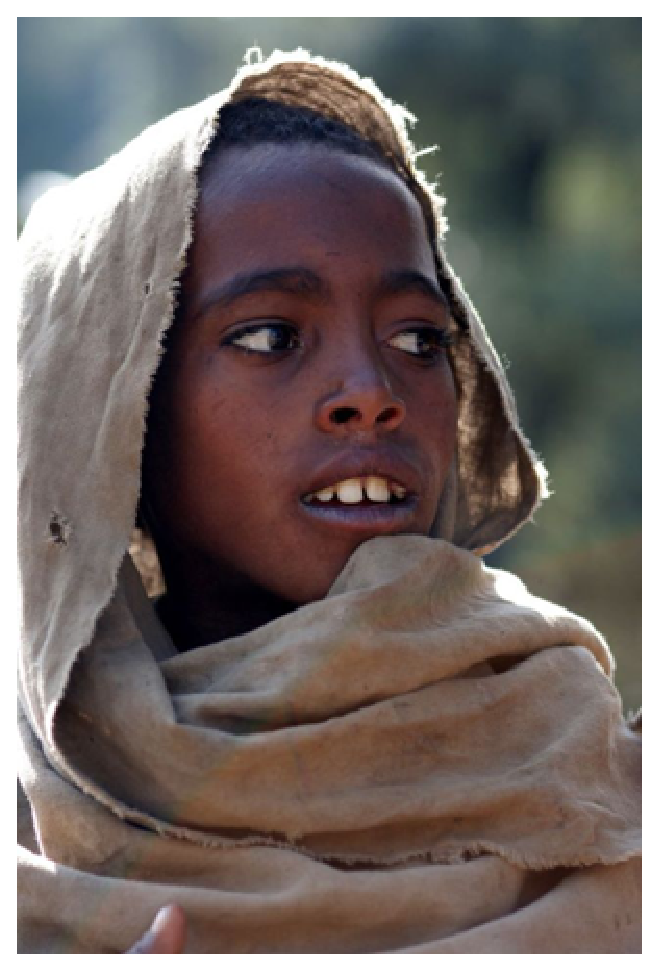
\includegraphics{etiopan.eps} \reflectbox{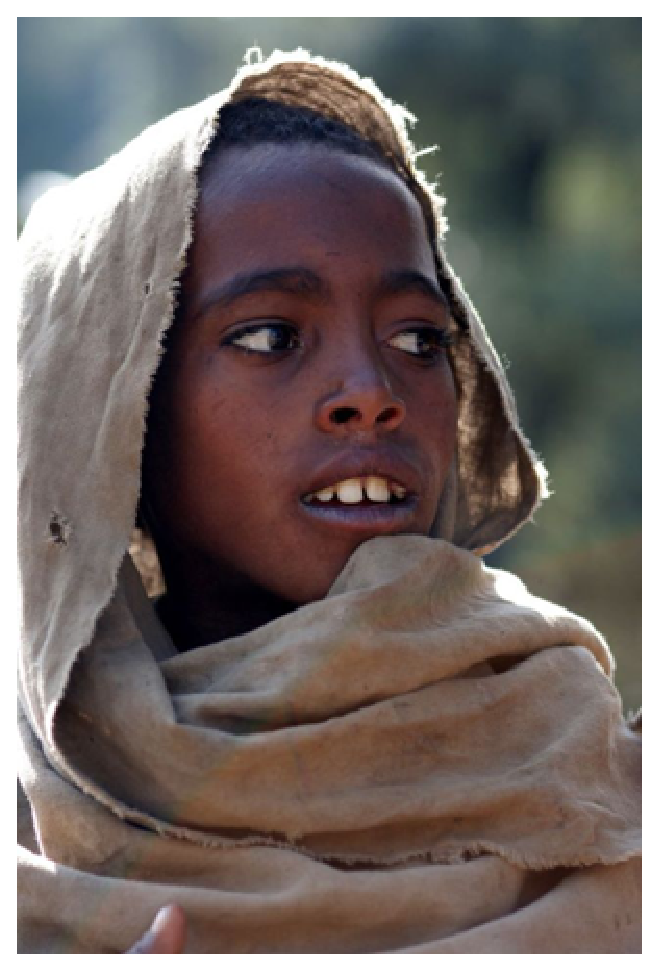
\includegraphics{etiopan.eps}}}
}
\label{import_picture}
\caption{Malý etiopánek a jeho bratříček}
\end{figure}
\newpage
Rozdíl mezi vektorovým \dots
\begin{figure}[h]
\center{\scalebox{0.35}{
\includegraphics{oniisan.eps}}}
\caption{Vektorový obrázek}
\label{vector_picture}
\end{figure}
\bigskip

\dots a bitmapovým obrázkem
\begin{figure}[h]
\center{\scalebox{0.65}{
\includegraphics{oniisan2.eps}}}
\caption{Bitmapový obrázek}
\label{bit_picture}
\end{figure}
\bigskip\\
se projeví například při zvětšení.

Odkazy (nejen ty) na obrázky \ref{import_picture}, \ref{vector_picture} a \ref{bit_picture}, na tabulky \ref{currency} a \ref{logic table} a také na algoritmus \ref{algorithm} jsou udělány pomocí křížových odkazů. Pak je ovšem potřeba zdrojový soubor přeložit dvakrát.

Vektorové obrázky lze vytvořit přímo v\LaTeX u i například pomocí prostředí \texttt{picture}.
\begin{landscape}
\begin{figure}

\begin{picture}(24cm,9.7cm)
                \setlength{\unitlength}{1cm}
                \linethickness{1pt}
                    
                    \linethickness{1pt}
                    \put(0,0){\line(1,0){24}}
                    \put(0,0){\line(0,1){9.7}}
                    \put(0,9.7){\line(1,0){24}}
                    \put(24,0){\line(0,1){9.7}}
                    \linethickness{5pt}
                    \put(0.4,1.4){\line(1,0){23}}
                    \put(0.4,1.2){\line(1,0){23}}
                    \put(0.4,1.6){\line(1,0){23}}
                    \put(0.4,1){\line(1,0){23}}
                    \put(0.4,0.8){\line(1,0){23}}
                    \put(0.4,0.6){\line(1,0){23}}

                    \linethickness{1pt}
                    \put(0.7,1.8){\line(1,0){14}}
                    \put(0.7,1.8){\line(0,1){5}}
                    \put(0.7,6.8){\line(1,1){2}}                       \put(2.7,8.8){\line(1,0){10}}
                    \put(14.7,6.8){\line(-1,1){2}}                  \put(14.7,1.8){\line(0,1){5}}
                    \put(0.7,6.8){\line(1,0){14}}
                    \put(1.7,1.8){\line(0,1){3}}                    \put(3.4,1.8){\line(0,1){3}}
                    \put(1.7,4.8){\line(1,0){1.7}}
                    \put(8,3){\line(0,1){2}}
                    \put(9.5,3){\line(0,1){2}}
                    \put(11,3){\line(0,1){2}}
                    \put(8,3){\line(1,0){3}}
                    \put(8,4){\line(1,0){3}}
                    \put(8,5){\line(1,0){3}}
                    \put(16,1.8){\line(0,1){4.5}}
                    \put(22,1.8){\line(0,1){4.5}}
                    \put(16,1.8){\line(1,0){6}}
                    \put(16,6.3){\line(1,0){6}}
                    \put(17.5,1.8){\line(0,1){2.5}}
                    \put(20.5,1.8){\line(0,1){2.5}}
                    \put(17.5,1.8){\line(1,0){3}}
                    \put(17.5,4.3){\line(1,0){3}}
                    \put(22.7,8.5){\circle{1.4}}

                \end{picture}

\caption{Vektorový obrázok nášho domu v prostredí \texttt{picture}.}
\label{picture}
\end{figure}
\end{landscape}
\end{document}
